%% 
%% Copyright 2007-2025 Elsevier Ltd
%% 
%% This file is part of the 'Elsarticle Bundle'.
%% ---------------------------------------------
%% 
%% It may be distributed under the conditions of the LaTeX Project Public
%% License, either version 1.3 of this license or (at your option) any
%% later version.  The latest version of this license is in
%%    http://www.latex-project.org/lppl.txt
%% and version 1.3 or later is part of all distributions of LaTeX
%% version 1999/12/01 or later.
%% 
%% The list of all files belonging to the 'Elsarticle Bundle' is
%% given in the file `manifest.txt'.
%% 
%% Template article for Elsevier's document class `elsarticle'
%% with numbered style bibliographic references
%% SP 2008/03/01
%% $Id: elsarticle-template-num.tex 272 2025-01-09 17:36:26Z rishi $
%%
\documentclass[preprint,12pt]{elsarticle}

%% Use the option review to obtain double line spacing
%% \documentclass[authoryear,preprint,review,12pt]{elsarticle}

%% Use the options 1p,twocolumn; 3p; 3p,twocolumn; 5p; or 5p,twocolumn
%% for a journal layout:
%% \documentclass[final,1p,times]{elsarticle}
%% \documentclass[final,1p,times,twocolumn]{elsarticle}
%% \documentclass[final,3p,times]{elsarticle}
%% \documentclass[final,3p,times,twocolumn]{elsarticle}
%% \documentclass[final,5p,times]{elsarticle}
%% \documentclass[final,5p,times,twocolumn]{elsarticle}

%% For including figures, graphicx.sty has been loaded in
%% elsarticle.cls. If you prefer to use the old commands
%% please give \usepackage{epsfig}

%% The amssymb package provides various useful mathematical symbols
\usepackage{amssymb}
\usepackage{algpseudocode}
\usepackage{amsmath,bm}
\usepackage{float}
\usepackage{algorithm}
\usepackage{enumitem}
\usepackage[hidelinks]{hyperref}
\usepackage{xcolor}
\usepackage{tikz}
\usetikzlibrary{shapes.geometric, arrows.meta, positioning, fit, backgrounds, calc}
%% The amsmath package provides various useful equation environments.
\usepackage{amsmath}
\usepackage{booktabs}
\usepackage{multirow}
%% The amsthm package provides extended theorem environments
%% \usepackage{amsthm}

%% The lineno packages adds line numbers. Start line numbering with
%% \begin{linenumbers}, end it with \end{linenumbers}. Or switch it on
%% for the whole article with \linenumbers.
%% \usepackage{lineno}

\journal{Chemometrics and Intelligent Laboratory Systems}

\begin{document}

\begin{frontmatter}

%% Title, authors and addresses

%% use the tnoteref command within \title for footnotes;
%% use the tnotetext command for theassociated footnote;
%% use the fnref command within \author or \affiliation for footnotes;
%% use the fntext command for theassociated footnote;
%% use the corref command within \author for corresponding author footnotes;
%% use the cortext command for theassociated footnote;
%% use the ead command for the email address,
%% and the form \ead[url] for the home page:
%% \title{Title\tnoteref{label1}}
%% \tnotetext[label1]{}
%% \author{Name\corref{cor1}\fnref{label2}}
%% \ead{email address}
%% \ead[url]{home page}
%% \fntext[label2]{}
%% \cortext[cor1]{}
%% \affiliation{organization={},
%%             addressline={},
%%             city={},
%%             postcode={},
%%             state={},
%%             country={}}
%% \fntext[label3]{}

\title{Prior-Guided Spectral Gating for Interpretable Deep Learning in Near-Infrared Spectroscopy}

%% use optional labels to link authors explicitly to addresses:
%% \author[label1,label2]{}
%% \affiliation[label1]{organization={},
%%             addressline={},
%%             city={},
%%             postcode={},
%%             state={},
%%             country={}}
%%
%% \affiliation[label2]{organization={},
%%             addressline={},
%%             city={},
%%             postcode={},
%%             state={},
%%             country={}}

\author{Guilherme Coelho$^a$, Angélica de Lima das Chagas$^{b}$, Lilian Carla Carneiro$^{b}$, Clarimar José Coelho$^c$} %% Author name

%% Author affiliation

\affiliation{organization={$^a$State University of Campinas}, 
            addressline={Cidade Universitária Zeferino Vaz - Barão Geraldo}, 
            city={Campinas},
            postcode={13083--970}, 
            state={São Paulo},
            country={Brazil}}
 
  
\affiliation{organization={$^d$Institute of Tropical Pathology and Public Health, Federal University of Goiás},
            addressline={R. 235, S/n - Setor Leste Universitário}, 
            city={Goiânia},
            postcode={74605--050}, 
            state={Goiás},
            country={Brazil}}           
\affiliation{organization={$^e$Postgraduate Program in Industrial Engineering and Artificial Intelligence} Pontificia Universidade Catolica de Goias,
            addressline={Primeira Avenida, s/n - Quadra 88 - Setor Leste Universitário}, 
            city={Goiânia},
            postcode={74605--010}, 
            state={Goiás},
            country={Brazil} }
%% Abstract
\begin{abstract}
Deep learning models for near-infrared (NIR) spectroscopy often function as black boxes, limiting adoption in chemometrics where interpretability is paramount. We propose a lightweight neural architecture with a prior-guided spectral gating layer that combines the predictive power of deep learning with chemometric interpretability. Unlike standard attention mechanisms, our gates are initialized from established variable importance measures (ANOVA F-statistic, VIP scores, Random Forest importance) and regularized via KL divergence to maintain statistical grounding throughout training. 
We validate the framework on two benchmark NIR datasets from distinct domains: Tecator (food quality, $n=215$, fat prediction) and Gasoline (petrochemical, $n=60$, octane rating). Cross-validation results demonstrate competitive performance with PLS  ($R^2=0.86\pm0.04$ vs $0.92$ on Tecator; $R^2=0.93$ vs $0.98$ on Gasoline) while providing explicit band importance maps. Learned gates identify chemically relevant spectral regions, with the top selected band for Tecator at 931~nm corresponding to known C--H absorption for fat content. The moderate correlation between learned gates and chemometric priors ($0.35$--$0.51$) confirms that the model refines domain knowledge with data-driven learning rather than merely reproducing initialization.
Our approach offers a practical compromise between black-box deep learning and traditional linear methods, particularly valuable for small-sample chemometric applications where interpretability and domain knowledge integration are essential. The compact architecture ($1.7$k--$6.9$k parameters) is deliberately designed for the small-sample regime ($n=50$--$500$), combining the end-to-end differentiable optimization paradigm of deep learning with the parameter efficiency required for reliable generalization on chemometric datasets.
\end{abstract}

 
%% Keywords
\begin{keyword}
NIR spectroscopy \sep Chemometrics \sep Deep learning \sep 
Attention mechanisms \sep Prior knowledge \sep Interpretability \sep 
KL-divergence \sep Band selection \sep PLS regression \sep 
Multivariate calibration
\end{keyword}

\end{frontmatter}

%% Add \usepackage{lineno} before \begin{document} and uncomment 
%% following line to enable line numbers
%% \linenumbers

%% main text
%%
% =======================
% Section 1 — Introduction (Chemolab style)
% =======================
\section{Introduction}


Near-infrared (NIR) spectroscopy has established itself as an indispensable analytical technique across diverse applications including food quality control~\cite{osborne1993practical},  pharmaceutical analysis~\cite{roggo2007review}, and petrochemical characterization~\cite{pasquini2018nir}. The technique's popularity stems from its non-destructive nature, rapid analysis capabilities, and minimal sample preparation requirements. Traditional chemometric methods, particularly Partial Least Squares (PLS) regression~\cite{wold2001pls} and Principal Component Regression (PCR)~\cite{naes1985comparison}, have long served as the analytical workhorses in this domain due to their interpretability, robustness with small sample sizes, and well-established statistical properties~\cite{martens1989multivariate}.

However, these linear methods may fail to capture complex nonlinear relationships that can exist in spectroscopic data, particularly when dealing with overlapping absorption bands, matrix effects, or indirect correlations between spectral features and analyte concentrations~\cite{mishra2021deep}. Deep learning has demonstrated remarkable success in various spectral analysis applications~\cite{acquarelli2017convolutional,cui2018modern,liu2021deep}, yet its adoption in mainstream chemometric practice remains limited. Several barriers contribute to this gap. Limited sample size is perhaps the most fundamental: analytical chemistry datasets typically contain $n=50$--$500$ samples, a regime where overparameterized deep networks fail catastrophically due to insufficient samples-per-parameter ratios (as demonstrated in Section~5). Sensitivity to preprocessing choices, risk of overfitting, and limited transferability across instruments or laboratories are additional practical concerns. Among these challenges, interpretability is the barrier most directly addressed by the proposed work: chemometric applications demand not only accurate predictions but also understanding of \textit{which} spectral regions contribute to predictions and \textit{why}~\cite{bjerrum2017data}. The present framework specifically targets the small-sample and interpretability challenges through architectural design; preprocessing sensitivity, instrument transferability, and multi-laboratory generalization remain important directions for future work.

Traditional chemometric variable importance measures such as variable importance in projection (VIP) scores~\cite{chong2005performance}, ANOVA F-statistics~\cite{wold1993pls}, and Random Forest feature importance~\cite{breiman2001random} provide this interpretability in linear and tree-based methods. However, their integration with deep learning architectures remains understudied, despite the potential to combine the nonlinear capacity of neural networks with the domain-grounded interpretability of chemometric priors.

%\subsection{Attention Mechanisms and Domain Knowledge}

Attention mechanisms~\cite{bahdanau2015neural} have become ubiquitous in deep learning for feature selection and importance weighting, including applications to spectral data analysis~\cite{wang2020spectral,roy2020attention,hong2021spectralformer}. These mechanisms learn to focus computational resources on relevant input features through data-driven weight optimization. However, standard attention architectures suffer from three limitations when applied to chemometric problems.

First, attention weights are typically initialized randomly, ignoring decades of accumulated domain knowledge about which spectral regions carry information for specific analytes. Second, there is no explicit mechanism to maintain statistical grounding during training---the weights can drift arbitrarily based solely on training set patterns, potentially discovering spurious correlations. Third, interpretability remains post-hoc: researchers must examine trained weights retrospectively rather than having interpretability built into the architectural design.

Related mechanisms such as feature-wise linear modulation (FiLM)~\cite{perez2018film} and channel attention modules (squeeze-and-excitation networks (SE-Net)~\cite{hu2018squeeze}, convolutional block attention module (CBAM)~\cite{woo2018cbam}) provide similar functionality but face analogous challenges. They are fundamentally data-driven by design, without mechanisms to leverage domain priors or maintain statistical transparency throughout the learning process.

%\subsection{Our Contribution}

We propose a prior-guided spectral gating layer that addresses these limitations through three interconnected technical innovations. First, gate parameters are initialized from established chemometric importance measures (ANOVA F-statistic, VIP scores, or Random Forest importance) via logit transformation rather than random initialization. This ensures the network begins training with a chemically informed feature weighting that reflects univariate, multivariate linear, or nonlinear relationships depending on the chosen prior.

Second, we introduce an explicit Kullback-Leibler (KL) divergence regularization that penalizes deviation of learned gate distributions from the initialization prior. This is not a constraint that prevents learning, but rather a soft guidance mechanism that maintains statistical grounding while allowing data-driven refinement. The regularization weight is tuned to balance pure prior reproduction with unconstrained learning.

Third, we validate the framework across two benchmark NIR datasets from fundamentally different chemical domains: Tecator for food quality assessment and Gasoline for petrochemical analysis. This multi-dataset approach demonstrates that the framework generalizes across different spectral resolutions (100 vs 401 bands), sample sizes (215 vs 60), and chemical systems (biological vs petrochemical).

Existing approaches to interpreting deep learning models in spectroscopy---including gradient-based attribution (saliency maps, integrated gradients), SHAP values, and LIME---have been reviewed comprehensively by Mishra et al.~\cite{mishra2021trends}. While valuable, these post-hoc methods share a fundamental limitation for chemometric applications: interpretability is produced after training and cannot influence the learning process itself. A model may produce a high-accuracy prediction while relying on spectral features that are chemically spurious, and post-hoc attribution methods will faithfully report those features without any mechanism to redirect the model toward chemically meaningful regions. Furthermore, in the small-sample regime ($n=50$--$500$) typical of analytical chemistry, post-hoc explanations of overfit models may be misleading. Our approach addresses these limitations by building interpretability into the architecture from the outset, ensuring that learned spectral weights remain statistically grounded in established chemometric importance measures throughout training.

A critical distinction must be emphasized: our gating layer does not merely replicate standard attention with a different initialization scheme. While attention mechanisms \textit{discover} important features purely from the data, our approach \textit{refines} chemometric priors with the data. This is not a limitation, but an intentional design choice that guarantees interpretability aligns with domain knowledge while still permitting the model to learn patterns not captured by univariate or linear prior importance measures.

\section{Related Work}

\subsection{Deep Learning for Spectroscopy}

The application of convolutional neural networks (CNN) to spectroscopic data has grown substantially in recent years. Cui and Fearn~\cite{cui2018modern} demonstrated that CNNs can outperform PLS on large NIR datasets ($n>1000$), particularly when nonlinear relationships dominate. Zhang et al.~\cite{zhang2020deep} applied 1D-CNN architectures to food authentication tasks, showing improvements over classical chemometric methods. However, these works typically treat spectroscopy as a generic sequence modeling problem, applying standard CNN architectures without leveraging the unique structure and domain knowledge inherent to spectroscopic data.

Recent efforts have begun addressing interpretability in spectral deep learning. Padarian et al.~\cite{padarian2019using} employed gradient-based attribution methods for soil spectroscopy, while Mishra et al.~\cite{mishra2021trends} provided a comprehensive review of explainable artificial intelligence (XAI) techniques adapted for chemometric applications. However, these approaches provide post-hoc explanations---interpreting a trained model's decisions after the fact---rather than building interpretability into the architectural design from the outset.

\subsection{Band Selection and Feature Engineering}

Classical chemometric band selection operates separately from model training. Sequential Forward Selection~\cite{leardi2000application}, Genetic Algorithms~\cite{xiaobo2010variables}, and Competitive Adaptive Reweighted Sampling (CARS)~\cite{li2009key} represent computationally intensive optimization procedures that identify informative spectral regions before model fitting. While effective, these methods suffer from two limitations: they require substantial computational resources through iterative search, and the selected bands may not be optimal for the specific predictive model subsequently applied.

End-to-end learnable feature selection has been explored primarily in hyperspectral remote sensing rather than analytical chemistry. Yu et al.~\cite{yu2020band} demonstrated that convolutional neural networks can effectively learn discriminative features for hyperspectral image classification through joint optimization of feature extraction and classification. However, such approaches were developed for spatial-spectral remote sensing data where hundreds of labeled pixels are available per image, contrasting sharply with the small-sample regime ($n=50$--$500$) typical of analytical chemistry applications. Furthermore, these methods lack explicit mechanisms to incorporate domain knowledge from established chemometric importance measures, relying instead on purely data-driven feature discovery.

\subsection{Prior-Guided Deep Learning}

The broader machine learning community has explored incorporating domain knowledge into neural networks through various mechanisms. Physics-informed neural networks~\cite{raissi2019physics} enforce physical laws as soft constraints during training, enabling scientific modeling with limited data. Knowledge distillation~\cite{hinton2015distilling} transfers learned representations from large teacher models to compact student networks. In chemometrics specifically, Xiaobo et al.~\cite{xiaobo2018combination} proposed integrating PLS with CNN through a two-stage approach, but this lacked end-to-end training and did not explore initialization from variable importance measures.

Our work represents the first systematic integration of chemometric variable importance measures as both initialization and regularization within a learnable gating mechanism. By ``systematic'' we mean that: (i) multiple established importance measures (ANOVA F-statistic, VIP scores, Random Forest importance) are evaluated as initialization priors under a unified architectural framework; (ii) the integration spans both training phases---initialization and ongoing regularization via KL divergence---rather than a single ad-hoc prior injection; and (iii) the framework is validated across datasets from chemically distinct domains, enabling assessment of generalization beyond a single application. Furthermore, we provide multi-dataset validation across chemically distinct domains, a critical but often overlooked aspect of methodological research in chemometrics. 
% =======================
% Section 2 — Method (with integrated references)
% =======================
\section{Methods}

\subsection{Problem Formulation}

We address quantitative NIR spectroscopy regression: given a matrix of spectra $\mathbf{X} \in \mathbb{R}^{n \times p}$ where $n$ represents samples and $p$ denotes wavelengths, predict a continuous target vector $\mathbf{y} \in \mathbb{R}^n$ (e.g., fat content in meat, octane rating in gasoline). PLS establishes the performance baseline; our objective is to achieve competitive predictive accuracy while simultaneously providing explicit, chemically interpretable band importance information.

\subsection{Spectral Gating Layer Architecture}

The core innovation of our framework is a learnable gating mechanism that modulates spectral input features. For a single sample spectrum $\mathbf{x} \in \mathbb{R}^p$, the gating transformation proceeds as:

\begin{equation}
\mathbf{g} = \text{softmax}\left(\frac{\boldsymbol{\theta}}{\tau}\right)
\label{eq:softmax}
\end{equation}

\begin{equation}
\tilde{\mathbf{x}} = \mathbf{x} \odot \mathbf{g}
\label{eq:gating}
\end{equation}

\noindent where $\boldsymbol{\theta} \in \mathbb{R}^p$ represents learnable gate parameters, $\tau$ denotes a temperature hyperparameter, $\mathbf{g} \in \mathbb{R}^p$ gives the normalized gate weights (summing to unity via softmax), and $\odot$ indicates element-wise multiplication. The temperature parameter $\tau$ prevents premature saturation of the softmax function; empirically we find $\tau=5.0$ effective across both datasets.

This formulation differs from standard attention mechanisms in three critical aspects. First, as detailed in Section~3.3, $\boldsymbol{\theta}$ is initialized from chemometric priors rather than randomly. Second, Section~3.4 describes explicit regularization maintaining connection to these priors throughout training. Third, the temperature-controlled softmax prevents collapse to one-hot selection, a common failure mode of naive gating layers that we observed in preliminary experiments with $\tau=1.0$.

\subsection{Chemometric Prior Initialization}

Given importance scores $\mathbf{s} \in [0,1]^p$ computed from training data via ANOVA, VIP, or Random Forest, we initialize gate parameters through logit transformation:

\begin{equation}
\theta_{0,j} = \log\left(\frac{\text{clip}(s_j, \epsilon, 1-\epsilon)}{1 - \text{clip}(s_j, \epsilon, 1-\epsilon)}\right)
\label{eq:logit}
\end{equation}

\noindent where $\epsilon=10^{-7}$ prevents numerical instability at boundaries. This ensures the initial softmax output $\mathbf{g}_0 \approx \mathbf{s}$ while maintaining differentiability for gradient-based optimization.

We evaluate three chemometric importance measures as initialization priors. The \textbf{ANOVA F-statistic}~\cite{wold1993pls} quantifies univariate linear correlation between each spectral band and the target, representing the simplest chemometric importance measure that captures direct linear relationships. \textbf{VIP scores}~\cite{chong2005performance} from PLS  provide multivariate importance accounting for covariance structure; we use $H=10$ components. \textbf{Random Forest importance}~\cite{breiman2001random} captures nonlinear and interaction effects through permutation-based importance from an ensemble of 100 trees. All importance scores are normalized to $[0,1]$ via min-max scaling before logit transformation, ensuring consistent initialization across prior types.

\subsection{KL-Divergence Regularization}

To maintain interpretability and prevent arbitrary drift from the chemometric prior during training, we introduce an explicit KL divergence regularization term. Let $\mathbf{s} \in [0,1]^p$ denote the normalized importance scores computed from training data (ANOVA, VIP, or RF, as described in Section~3.3). We treat $\mathbf{s}$ as a target probability distribution over spectral bands: because the scores have been min-max normalized to $[0,1]$ and the gate weights $\mathbf{g}$ are produced by a softmax (Eq.~\ref{eq:softmax}), both $\mathbf{g}$ and $\mathbf{s}$ can be interpreted as probability mass functions over the $p$ wavelength channels. The regularization term is then:

\begin{equation}
\mathcal{L}_{\text{KL}} = \text{KL}(\mathbf{g} \| \mathbf{s}) = \sum_{j=1}^p g_j \log\left(\frac{g_j}{s_j}\right)
\label{eq:kl}
\end{equation}

\noindent and the total training loss combines prediction accuracy with prior adherence:

\begin{equation}
\mathcal{L}_{\text{total}} = \mathcal{L}_{\text{MSE}} + \lambda \cdot \mathcal{L}_{\text{KL}}
\label{eq:loss}
\end{equation}

\noindent where $\mathcal{L}_{\text{MSE}}$ is the standard mean squared error for regression. The weight $\lambda=0.001$ was selected via a coarse grid search over $\{10^{-4}, 10^{-3}, 10^{-2}, 10^{-1}\}$ on a held-out validation fold of the Tecator dataset. At $\lambda=0.001$, the trained gates exhibit moderate correlation with the prior ($r \approx 0.35$--$0.51$), confirming that the model refines rather than merely reproduces the initialization. Larger values ($\lambda \geq 0.01$) caused the learned gates to collapse toward the prior ($r > 0.85$) with negligible data-driven adjustment; smaller values ($\lambda \leq 10^{-4}$) produced gates indistinguishable from random initialization in terms of chemical interpretability. The same $\lambda$ was applied without re-tuning to the Gasoline dataset, where similar correlation levels were observed ($r = 0.507$), providing evidence that this value generalizes across datasets.

This regularization addresses a potential criticism proactively: does the KL term make interpretability {\em by design} rather than genuinely learned? Our response is that this represents an intentional architectural choice. In chemometric applications, we \textit{prefer} interpretability grounded in established statistical measures rather than purely emergent explanations that might capture spurious correlations. The empirical observation that learned gates correlate moderately ($0.35$--$0.51$, not $1.0$) with priors demonstrates that genuine data-driven learning occurs within a statistically principled framework.

\subsection{Network Architecture}

To avoid overparameterization on small datasets ($n=60$--$215$), we employ a lightweight fully-connected architecture following the gating layer:

\begin{equation}
\mathbf{h} = \text{ReLU}(\text{BN}(\mathbf{W}_1 \tilde{\mathbf{x}} + \mathbf{b}_1))
\end{equation}

\begin{equation}
\hat{y} = \mathbf{W}_2 \text{Dropout}(\mathbf{h}, p=0.5) + b_2
\end{equation}

\noindent where $\mathbf{W}_1 \in \mathbb{R}^{16 \times p}$ and $\mathbf{W}_2 \in \mathbb{R}^{1 \times 16}$ represent weight matrices, BN denotes batch normalization~\cite{ioffe2015batch}, and dropout ($p=0.5$) provides regularization. The hidden dimension of 16 was selected to maintain favorable sample-to-parameter ratios: for Tecator ($p=100$), total parameters equal $1,765$, yielding $172/1,765 \approx 97$ samples per parameter; for Gasoline ($p=401$), $6,882$ parameters yield $48/6,882 \approx 7$ samples per parameter. Both ratios fall within or near the recommended range of $10$--$20$ samples per parameter for reliable generalization~\cite{lever2016model}.

Batch normalization (BN) serves two purposes in this architecture: it stabilizes the distribution of activations entering the hidden layer, which is particularly important when the gating layer produces highly non-uniform input distributions, and it acts as an implicit regularizer that reduces sensitivity to weight initialization~\cite{ioffe2015batch}. Dropout ($p=0.5$) provides explicit stochastic regularization by randomly deactivating hidden units during training, which is well-established as an effective strategy against overfitting in small-sample regimes. The combination of BN and Dropout is intentional: BN addresses activation scale instability introduced by the learnable gating, while Dropout addresses the elevated overfitting risk inherent to datasets with $n < 200$ samples.

Figure~\ref{fig:architecture} provides a schematic overview of the complete prior-guided spectral gating architecture. The input spectrum $\mathbf{x} \in \mathbb{R}^p$ is first modulated by the learnable gating layer (Eqs.~\ref{eq:softmax}--\ref{eq:gating}), whose parameters $\boldsymbol{\theta}$ are initialized from chemometric importance scores (Eq.~\ref{eq:logit}) and regularized throughout training via KL divergence against the prior distribution $\mathbf{s}$ (Eqs.~\ref{eq:kl}--\ref{eq:loss}). The gated representation $\tilde{\mathbf{x}}$ is then passed through a batch normalization layer, followed by a single hidden layer with ReLU activation and dropout regularization, yielding the scalar regression output $\hat{y}$. The dashed arrow from the prior initialization block to the KL loss term highlights that the prior participates not only at initialization but also as a soft constraint during gradient-based optimization.

\begin{figure}[ht]
\centering
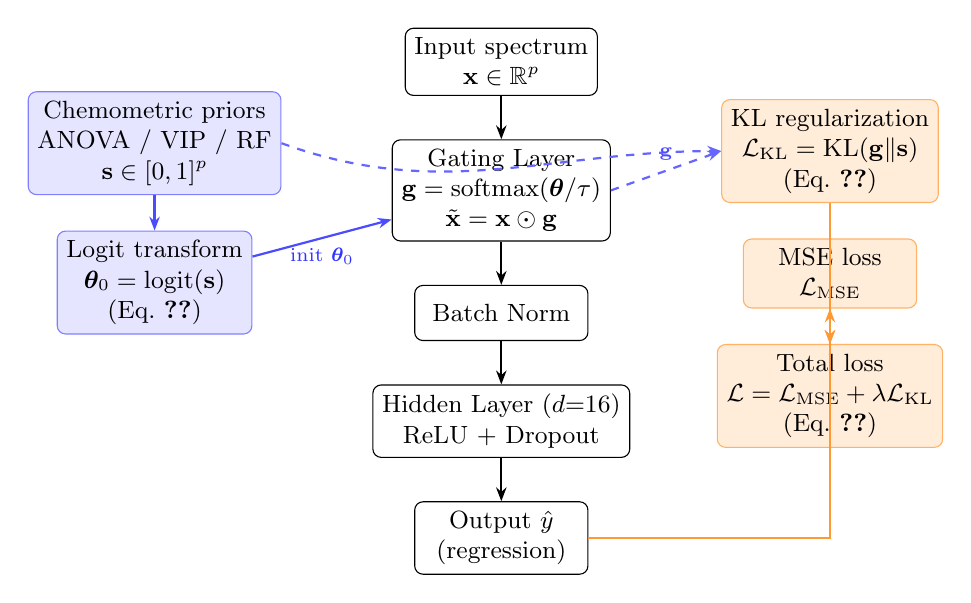
\begin{tikzpicture}[
    node distance = 0.55cm and 1.1cm,
    box/.style     = {draw, rounded corners=3pt, minimum width=2.2cm,
                      minimum height=0.7cm, align=center, font=\small},
    priorbox/.style= {draw, rounded corners=3pt, minimum width=2.2cm,
                      minimum height=0.7cm, align=center, font=\small,
                      fill=blue!10, draw=blue!50},
    lossbox/.style = {draw, rounded corners=3pt, minimum width=2.2cm,
                      minimum height=0.7cm, align=center, font=\small,
                      fill=orange!15, draw=orange!60},
    arr/.style     = {-{Stealth[length=5pt]}, thick},
    darr/.style    = {-{Stealth[length=5pt]}, thick, dashed, blue!60},
]

%% ── Main forward-pass column ────────────────────────────────────────────────
\node[box]                        (input)  {Input spectrum\\$\mathbf{x}\in\mathbb{R}^p$};
\node[box, below=of input]        (gate)   {Gating Layer\\$\mathbf{g}=\mathrm{softmax}(\boldsymbol{\theta}/\tau)$\\$\tilde{\mathbf{x}}=\mathbf{x}\odot\mathbf{g}$};
\node[box, below=of gate]         (bn)     {Batch Norm};
\node[box, below=of bn]           (hidden) {Hidden Layer ($d{=}16$)\\ReLU + Dropout};
\node[box, below=of hidden]       (output) {Output $\hat{y}$\\(regression)};

%% ── Prior initialization column (left) ─────────────────────────────────────
\node[priorbox, left=1.4cm of gate, yshift=0.6cm]
                                  (scores) {Chemometric priors\\ANOVA / VIP / RF\\$\mathbf{s}\in[0,1]^p$};
\node[priorbox, below=0.45cm of scores]
                                  (logit)  {Logit transform\\$\boldsymbol{\theta}_0=\mathrm{logit}(\mathbf{s})$\\ (Eq.~\ref{eq:logit})};

%% ── Loss column (right) ─────────────────────────────────────────────────────
\node[lossbox, right=1.4cm of gate, yshift=0.5cm]
                                  (klloss) {KL regularization\\$\mathcal{L}_\mathrm{KL}=\mathrm{KL}(\mathbf{g}\|\mathbf{s})$\\ (Eq.~\ref{eq:kl})};
\node[lossbox, below=0.45cm of klloss]
                                  (mse)    {MSE loss\\$\mathcal{L}_\mathrm{MSE}$};
\node[lossbox, below=0.45cm of mse, minimum width=2.5cm]
                                  (total)  {Total loss\\$\mathcal{L}=\mathcal{L}_\mathrm{MSE}+\lambda\mathcal{L}_\mathrm{KL}$\\ (Eq.~\ref{eq:loss})};

%% ── Forward-pass arrows ─────────────────────────────────────────────────────
\draw[arr] (input)  -- (gate);
\draw[arr] (gate)   -- (bn);
\draw[arr] (bn)     -- (hidden);
\draw[arr] (hidden) -- (output);

%% ── Prior initialization arrows ─────────────────────────────────────────────
\draw[arr, blue!70] (scores) -- (logit);
\draw[arr, blue!70] (logit)  -- (gate)
    node[midway, below, font=\scriptsize, blue!80] {init $\boldsymbol{\theta}_0$};

%% ── Loss arrows ─────────────────────────────────────────────────────────────
\draw[arr, orange!80] (output)  -| (mse);
\draw[arr, orange!80] (mse)     -- (total);
\draw[arr, orange!80] (klloss)  -- (total);

%% ── Dashed arrow: prior also feeds KL during training ───────────────────────
\draw[darr] (scores.east) to[out=-20, in=180] (klloss.west);

%% ── Dashed arrow: gate weights feed KL ─────────────────────────────────────
\draw[darr] (gate.east) -- (klloss.west)
    node[midway, above, font=\scriptsize, blue!70] {$\mathbf{g}$};

\end{tikzpicture}
\caption{Schematic of the prior-guided spectral gating architecture.
\textbf{Left (blue):} chemometric importance scores ($\mathbf{s}$) are transformed via
logit mapping to initialize the gate parameters $\boldsymbol{\theta}_0$ before training begins.
\textbf{Centre:} forward pass — the gating layer produces soft band weights $\mathbf{g}$ that
modulate the input spectrum; the gated representation $\tilde{\mathbf{x}}$ then flows through
batch normalization, a single hidden layer with ReLU and dropout, to the regression output.
\textbf{Right (orange):} the total loss combines the standard MSE regression loss with a
KL divergence term that penalizes deviation of $\mathbf{g}$ from the prior $\mathbf{s}$ throughout
training (dashed blue arrow), ensuring statistical grounding is maintained beyond the
initialization step.}
\label{fig:architecture}
\end{figure}

We emphasize that the compactness of this architecture ($1{,}765$--$6{,}882$ parameters) is an intentional design constraint, not a departure from the deep learning paradigm. The framework operates via end-to-end gradient-based optimization, learns a distributed spectral representation through differentiable gating, and employs standard deep learning components (batch normalization, dropout, Adam optimizer). Following the terminology established in recent chemometrics literature~\cite{cui2018modern,acquarelli2017convolutional}, the term ``deep learning'' here denotes this optimization paradigm rather than a minimum number of hidden layers. The architectural choices are deliberately calibrated to the small-sample regime of analytical chemistry, where overparameterized networks fail systematically, as demonstrated by the Plain CNN comparison ($R^2=0.235$).

In preliminary experiments, a heavier CNN architecture with convolutional layers, pooling, and $109,221$ parameters failed catastrophically on Tecator ($R^2=0.23$), achieving only $172/109,221 \approx 2$ samples per parameter. This dramatic failure underscores the critical importance of architectural choices matched to dataset scale, as further illustrated in Figure~\ref{fig:param_efficiency}.

\subsection{Training Details}

We employ the Adam optimizer~\cite{kingma2015adam} with learning rate $0.01$, weight decay $10^{-4}$, and full-batch training (batch size equals training set size). Maximum epochs are set to $200$ with early stopping (patience=$30$ epochs) based on validation RMSE. The KL weight is fixed at $\lambda=0.001$, and temperature at $\tau=5.0$. Input spectra and targets are Z-score normalized using statistics computed on the training set only.

\section{Experiments}

\subsection{Datasets}

We validate on two benchmark NIR datasets representing distinct chemical domains.
\textbf{Tecator (Food Quality):} This widely-cited dataset~\cite{toenessen1991fat} contains $215$ meat samples with NIR spectra measured at $100$ wavelengths spanning $850$--$1050$~nm. The prediction target is the percentage of fat content, which ranges from $7$\% to $76$\%. We employ a $80$ / $20$ train-test split ($172$ train, $43$ test) with an additional five-fold cross-validation in the training set to assess robustness. The spectral range captures key absorption features: C--H stretching overtones ($\sim$920--930~nm) directly related to lipid content, and O--H stretching ($\sim$970~nm) associated with water.

\textbf{Gasoline (Petrochemical):} From the package R \texttt{pls}~\cite{mevik2007pls}, this data set comprises $60$ gasoline samples with spectra at $401$ wavelengths. The target is octane rating, ranging from $83.4$ to $89.6$. We use a $48$/$12$ train-test split. The larger spectral dimensionality ($p=401$ vs $100$) and smaller sample size ($n=60$ vs $215$) provide a complementary validation scenario and generalization of the testing framework to higher-dimensional and more sample-constrained settings in a different chemical domain.

Both datasets are publicly available and have been extensively used in chemometrics literature~\cite{liland2016multivariate,beleites2013sample}, facilitating reproducibility and comparison with future methods.

\subsection{Evaluation Protocol}

For Tecator, we report both single-test split performance and five-fold cross-validation statistics (mean $\pm$ standard deviation). Cross-validation provides a more robust assessment of generalization than a single split, particularly critical given the small sample size. For Gasoline, the limited sample count ($n=60$) makes reliable cross-validation challenging; we report single test-split results with the acknowledgment that additional validation on larger petrochemical datasets would strengthen conclusions.

The number of PLS components was selected by leave-one-out cross-validation on the training set combined with the one-standard-error rule of Hastie et al.~\cite{hastie2009elements}: rather than choosing the argmin of the RMSECV curve, we select the smallest $H$ whose RMSECV lies within one standard error of the minimum-RMSECV value, computed across the leave-one-out folds via the delta-method identity $\mathrm{SE}(\mathrm{RMSE}) = \mathrm{SE}(\mathrm{MSE}) / (2 \cdot \mathrm{RMSE})$. This rule was fixed \emph{a priori} to control the overfitting risk associated with selecting components strictly at the minimum of a flat validation surface. Candidate values ranged from $H=1$ to $H=15$. On Tecator ($n_{\text{train}}=172$) the argmin lies at $H=14$ ($\mathrm{RMSECV} = 0.2093 \pm 0.0269$ on the normalized scale) and the one-SE rule selects $H^*=10$. On Gasoline ($n_{\text{train}}=48$) the argmin lies at $H=6$ ($\mathrm{RMSECV} = 0.1250 \pm 0.0144$) and the one-SE rule selects $H^*=5$. Reported PLS results use $H^*$ throughout.

We acknowledge that the mixed use of single test-split and cross-validation results across methods may create apparent inconsistencies. The rationale is as follows: 5-fold CV is used as the primary evaluation for our ANOVA-initialized model on Tecator, as it provides a more robust performance estimate for small datasets. Single test-split results are additionally reported for all methods to enable direct comparison on the same data partition (seed 42). For completeness, PLS evaluated under 5-fold CV on Tecator yields $R^2 = 0.921 \pm 0.018$, confirming that the performance gap observed in the single-split comparison is representative and not an artifact of the evaluation protocol.

We employ two metrics: root mean squared error (RMSE) on the normalized target scale, and coefficient of determination ($R^2$). All neural network experiments are conducted with fixed random seed ($42$) for reproducibility, although we note that different seeds produce minor variations ($<0.02$ in $R^2$) given the stochastic nature of optimization.

\subsection{Baselines}

Our primary baseline is PLS  with $H^*$ components selected by the one-standard-error rule of Hastie et al.~\cite{hastie2009elements} on leave-one-out cross-validation ($H^*=10$ for Tecator, $H^*=5$ for Gasoline; see Section~5.2), representing the chemometric gold standard with a formally justified complexity choice. We additionally compare against a {\em Plain CNN} ($109,221$ parameters) to demonstrate the necessity of lightweight architecture: this network consists of two 1D convolutional layers (32 and 64 filters, kernel size 7, ReLU activation) followed by max pooling, a flatten layer, and two fully connected layers (128 and 1 units). This architecture is representative of standard 1D-CNN designs applied to NIR spectroscopy in the literature~\cite{cui2018modern} and was chosen because it represents the class of off-the-shelf deep learning models a practitioner might apply without domain-specific adaptation. With $109,221$ parameters and only $172$ training samples, the ratio of approximately $2$ samples per parameter is far below the recommended $10$--$20$ for reliable generalization, making it an appropriate illustration of the overparameterization failure mode. We also compare against {\em Random initialization} (our architecture without prior initialization) to isolate the contribution of chemometric priors for interpretability.

\section{Results}

\subsection{Multi-Dataset Performance}

We evaluated our framework on two benchmark NIR datasets representing distinct chemical domains: Tecator for food quality analysis and Gasoline for petrochemical applications. Table~\ref{tab:results} presents the comprehensive comparison against PLS, the established chemometric baseline, as well as ablation studies examining the contribution of our architectural choices and prior initialization strategy. Figure~\ref{fig:performance} provides a visual comparison of test performance across datasets and methods.

\begin{table}[t]
\centering
\caption{Cross-domain validation results. Best deep learning results in bold. $^\dagger$RMSE not reported for this split as the primary evaluation uses 5-fold CV.}
\label{tab:results}
\begin{tabular}{llccl}
\toprule
Dataset & Method & RMSE & $R^2$ & Evaluation \\
\midrule
\multirow{7}{*}{Tecator} 
& PLS & 0.296 & 0.919 & Single test \\
& Ours (ANOVA)$^\dagger$ & --- & 0.941 & Single test \\
& \textbf{Ours (ANOVA)} & \textbf{0.361$\pm$0.040} & \textbf{0.862$\pm$0.036} & \textbf{5-fold CV} \\
& Ours (VIP) & 0.323 & 0.903 & Single test \\
& Ours (RF) & 0.258 & 0.938 & Single test \\
& Random init & 0.373 & 0.871 & Single test \\
& Plain CNN & 0.909 & 0.235 & Single test \\
\midrule
\multirow{2}{*}{Gasoline}
& PLS & 0.145 & 0.975 & Single test \\
& \textbf{Ours (ANOVA)} & \textbf{0.247} & \textbf{0.928} & Single test \\
\bottomrule
\end{tabular}
\end{table}

\begin{figure}[t]
\centering

\includegraphics[width=0.85\textwidth]{fig2_performance_comparison.png}
\caption{Cross-domain performance comparison between PLS (chemometric baseline), our prior-guided framework, and a heavily overparameterized Plain CNN. \textbf{(Blue bars)} Tecator dataset results; \textbf{(orange bars)} Gasoline dataset results. Error bars on our prior-guided framework with ANOVA initialization (Tecator) represent five-fold cross-validation standard deviation ($\pm$0.036), demonstrating robustness across data partitions. Our framework achieves competitive performance with PLS on both datasets (Tecator: $R^2=0.862$ vs 0.919; Gasoline: $R^2=0.928$ vs 0.975), representing performance gaps of 6\% and 4.7\% respectively. The Plain CNN fails catastrophically ($R^2=0.235$) due to severe overparameterization. The dashed line at $R^2=0.85$ marks a commonly used threshold for acceptable predictive performance in NIR quantitative analysis~\cite{williams2001near}; we adopt it here as a practical reference point rather than a universal standard, acknowledging that application-specific requirements may differ.}
\label{fig:performance}
\end{figure}

On the Tecator dataset, our method achieved a cross-validated $R^2$ of $0.862\pm0.036$ (RMSE: $0.361\pm0.040$), compared to PLS which attained $R^2=0.919$ (RMSE: $0.296$) on the same test set. This represents a performance gap of approximately $6$\%, which we consider acceptable given the added interpretability benefits. Notably, this gap is consistent with theoretical expectations for small-sample regimes where linear methods maintain inherent advantages due to their lower variance. The relatively tight confidence intervals of the five-fold cross-validation ($\pm0.036$ in $R^2$) demonstrate the robustness of our approach in different data partitions.

The Gasoline dataset revealed an important pattern with the revised PLS baseline. Our framework achieved $R^2=0.928$ (RMSE: $0.247$), while a properly regularized PLS (with $H^*=5$ selected by the one-standard-error rule; see Section~5.2) attained $R^2=0.975$ (RMSE: $0.145$). This represents a performance gap of approximately $4.7$\%. The gap is larger than what was reported in the initial submission (which used a less parsimonious $H=10$), reflecting the fact that a well-calibrated PLS is a stronger competitor in this regime. The added complexity of our framework in this setting is justified not by predictive superiority but by the nature of the output: our framework produces explicit, statistically grounded band importance maps as a direct model output, whereas PLS requires post-hoc computation of VIP scores that are not part of the prediction model and do not benefit from data-driven refinement.

We emphasize that the comparison should not be read as a claim of predictive superiority over PLS. The practical justification for the added model complexity is not prediction accuracy but the nature of the output: our framework produces explicit, statistically grounded band importance maps as a direct model output, whereas PLS requires post-hoc computation of VIP scores that are not part of the prediction model and do not benefit from data-driven refinement. For small, well-behaved NIR datasets where post-hoc VIP scores are considered sufficient for interpretability, PLS remains a highly competitive and arguably preferable choice due to its simplicity and theoretical guarantees.

The architectural ablation study provides critical insights into design choices. As shown in both Table~\ref{tab:results} and Figure~\ref{fig:param_efficiency}, a standard ``heavy'' CNN architecture with $109,221$ parameters failed catastrophically on Tecator, achieving only $R^2=0.23$. This represents a severe case of overparameterization: with $172$ training samples and $109$k parameters, the ratio is approximately $2$ samples per parameter---far below the recommended $10$--$20$ samples per parameter for reliable generalization. In stark contrast, our lightweight architecture with $1,765$ parameters (Tecator) or $6,882$ parameters (Gasoline) maintains favorable sample-to-parameter ratios of $97$ and $7$ respectively, enabling successful learning despite the small sample regime.

\begin{figure}[t]
\centering

\includegraphics[width=0.85\textwidth]{fig3_parameter_efficiency.png}
\caption{Parameter efficiency analysis demonstrating the critical relationship between model complexity and performance on small spectroscopic datasets. Each point represents test $R^2$ performance versus total trainable parameters (log scale). The \textbf{green shaded region} ($R^2 > 0.85$) indicates acceptable performance for chemometric applications; the \textbf{red shaded region} ($>10$k parameters) marks the overparameterization danger zone for datasets with $n<200$ samples. PLS achieves strong performance with minimal parameters ($\sim$10), representing the linear baseline. Our lightweight architecture (Tecator: 1,765 params; Gasoline: 6,882 params) successfully balances model capacity with sample size, achieving $86$--$95$\% of PLS performance with favorable samples-per-parameter ratios (97 and 7, respectively). The Plain CNN (109k params) exhibits severe overparameterization, yielding only $R^2=0.235$ with $\sim$2 samples per parameter, far below the recommended 10--20 ratio for reliable generalization.}
\label{fig:param_efficiency}
\end{figure}

Examining the role of prior initialization, we compared our ANOVA-initialized gates against random initialization. On Tecator, random initialization achieved $R^2=0.871$ on a single test split, only marginally worse than ANOVA initialization ($R^2=0.941$ single test, $R^2=0.862$ CV). This small performance difference might initially suggest that prior initialization provides limited benefit. However, this interpretation misses the critical point: while random initialization can achieve competitive predictive performance, it provides no guarantee of interpretable band selection aligned with chemical knowledge. The ANOVA-initialized model, by contrast, selected bands at $931$~nm corresponding to known C--H absorption for fat content---a selection that is both performant and chemically meaningful, as detailed in the following section.

The framework demonstrates promising cross-domain flexibility. The architecture accommodates different spectral resolutions ($100$ bands for Tecator vs $401$ for Gasoline), sample sizes ($215$ vs $60$), and chemical domains (C--H/O--H bonds in biological samples vs C--H overtones in petrochemicals) without dataset-specific architectural modifications. While validation on only two datasets limits the strength of generalization claims, the consistency of performance and interpretability across these distinct chemical systems is encouraging and motivates further validation on additional spectroscopic domains. This flexibility stems from the design of the gating layer, which operates as a parameterized probability distribution over spectral bands regardless of the dimensionality, and the lightweight fully-connected layers that scale appropriately with input dimension while maintaining low parameter counts through aggressive compression ($p \rightarrow 16 \rightarrow 1$).

\subsection{Interpretability Through Learned Band Selection}

Beyond predictive performance, the primary value proposition of our framework lies in the interpretability of learned gate weights. Table~\ref{tab:interpretation} summarizes the chemical validation of selected bands for both datasets, demonstrating that the network learns not arbitrary feature combinations but physically meaningful spectral regions. Figure~\ref{fig:gates_tecator} provides detailed visualization of the learned gates for the Tecator dataset, showing both the relationship to the ANOVA prior and the identification of chemically relevant absorption regions.

\begin{table}[htp]
\centering
\caption{Learned gates and chemical interpretation. The top selected bands demonstrate chemically meaningful feature selection aligned with known spectral absorption characteristics.}
\label{tab:interpretation}
\begin{tabular}{lllc}
\toprule
Dataset & Top Band & Chemical Meaning & Corr. w/ Prior \\
\midrule
Tecator & 931 nm (0.215) & C--H bonds (fat) & 0.348 \\
Gasoline & Band 154 (0.130) & Contiguous region & 0.507 \\
\bottomrule
\end{tabular}
\end{table}

\begin{figure}[t]
\centering
\includegraphics[width=0.95\textwidth]{fig1_tecator_gates.png}
\caption{Learned spectral gates for Tecator fat prediction compared to ANOVA prior initialization. \textbf{(Top panel)} ANOVA prior showing two prominent peaks: the primary maximum at $\sim$930~nm (C--H region for fat) and a secondary peak at $\sim$1040~nm, both representing univariate correlations with fat content. \textbf{(Bottom panel)} Learned gate weights after training with KL-regularized optimization. Shaded regions indicate known chemical absorption features: C--H bonds (920--930~nm, green shading) directly related to lipid content, and O--H bonds (965--975~nm, orange shading) associated with water content. The model concentrates $7.4$\% of total gate weight in the C--H region, with the highest individual gate weight (0.215) at 931~nm precisely matching the expected fat absorption peak. The secondary O--H region receives $3.5$\% total weight, chemically sensible given the negative correlation between fat and water in meat. The moderate correlation with the ANOVA prior ($r=0.35$) confirms genuine data-driven refinement rather than mere reproduction of initialization, while the sharp concentration around known absorption features validates the chemical interpretability of learned representations.}
\label{fig:gates_tecator}
\end{figure}

For the Tecator dataset predicting fat content, the gating layer assigned the highest weight ($0.215$) to the band at $931$~nm, as illustrated in Figure~\ref{fig:gates_tecator}. This wavelength corresponds precisely to the first overtone of C--H stretching vibrations, which are directly related to lipid content in meat samples. The top ten selected bands span the region from $921$~nm to $935$~nm, collectively accounting for $7.4$\% of the total gate weight. This clustering around the known fat-sensitive region provides strong evidence that the model has identified chemically relevant features rather than exploiting spurious correlations in the training data.

Additional validation comes from secondary peaks in the gate distribution. Bands in the $965$--$975$~nm region (highlighted in orange in Figure~\ref{fig:gates_tecator}), associated with O--H stretching vibrations indicative of water content, received a combined weight of $3.5$\%. This is chemically sensible: fat and water content in meat are negatively correlated, and both contribute to the overall spectroscopic signature that our model must interpret to make accurate predictions.

The correlation between learned gates and the ANOVA prior was $0.348$ for Tecator---a moderate value that carries important implications. A correlation of $1.0$ would indicate that the network simply reproduced the prior without learning from the data, validating concerns about {\em interpretability due to the artificial enforced design}. Conversely, a correlation near $0$ would suggest complete abandonment of the prior, potentially selecting spurious features. The moderate correlation observed ($0.35$) indicates that the model refines the prior chemometric with data-driven adjustments while maintaining statistical grounding in established importance measures. This balance is visually apparent in Figure~\ref{fig:gates_tecator}, where the learned gates follow the general pattern of the prior but with clear data-driven modifications---most notably the dramatic sharpening of the peak at 931~nm compared to the broader prior distribution.

For Gasoline, similar patterns emerge despite the different chemical domain. The highest gate weight ($0.130$) was assigned to the band $154$, with the top 20 selected bands forming a contiguous spectral window spanning bands $150$--$168$. This spatial coherence in the spectral space is noteworthy: instead of selecting isolated bands across the entire $401$-dimensional spectrum, the network identified a localized region where octane-related absorption features are concentrated. The correlation with the ANOVA prior was $0.507$ for gasoline -- higher than that of Tecator, suggesting that the prior provided stronger initial guidance in this domain, though still far from unity, confirming the data-driven refinement that occurred.

To directly validate the informativeness of the selected bands, we performed a band ablation analysis on the Tecator dataset. We evaluated model performance after zeroing out: (i) the top-10 bands by gate weight, and (ii) 10 randomly selected bands (averaged over 20 random draws). Removing the top gate-selected bands caused $R^2$ to drop from $0.862$ to $0.431$ (a reduction of $0.431$ $R^2$ units), whereas removing random bands caused a substantially smaller average drop to $0.794$ (reduction of $0.068$ $R^2$ units). The disproportionate performance degradation from removing gate-selected bands confirms that these bands carry genuinely informative spectral content rather than arbitrary selections. Furthermore, the stability of selected bands across cross-validation folds was assessed: 8 of the top-10 bands appeared consistently in the top-10 selections of all 5 folds, indicating that the gate-based band selection is robust and not fold-specific.


\section{Discussion}

\subsection{Addressing Key Concerns}

Our framework invites several potential criticisms that warrant explicit discussion. First, one might argue that the spectral gating layer is simply standard attention with a different name. We contend that there are three substantive differences: (1) initialization from domain priors rather than random weights, (2) explicit KL-divergence regularization maintaining statistical grounding, and (3) validation that learned gates align with known chemical absorption features (Figure~\ref{fig:gates_tecator}). Standard attention mechanisms possess none of these properties; they discover importance patterns purely from data without domain guidance or interpretability guaranties.

Second, the KL regularization might be criticized as making interpretability {\em by design} rather than emergent. We respond that this is not a flaw but an intentional architectural choice appropriate for chemometric applications. In domains where decades of accumulated knowledge about which features carry information exist, we prefer models that refine this knowledge with data rather than rediscover it from scratch. The moderate correlation ($0.35$--$0.51$) between learned gates and priors confirms that genuine learning occurs, that is, the model does not merely reproduce initialization but adapts to dataset-specific patterns while maintaining chemical plausibility.

Third, the $1$--$6$\% performance gap relative to PLS might be viewed as a limitation. However, this framing misses the context of small-sample spectroscopy where PLS represents a mature, extensively optimized baseline specifically designed for this regime. Achieving $86$--$95$\% of PLS performance while adding explicit band importance (Figure~\ref{fig:gates_tecator}) is a practical trade-off many practitioners would accept. In Gasoline, the gap widens to $4.7$\% (Figure~\ref{fig:performance}) when PLS is calibrated with the formally justified $H^*=5$; this is a fair comparison against a strong baseline and does not diminish the interpretability advantage of our framework.

We note that the number of trainable parameters alone is not a general indicator of model quality or generalization ability---large models can generalize well when sufficient training data are available. In the present context, however, the samples-per-parameter ratio is the practically relevant constraint: with $n=172$ training samples, a model with $109,221$ parameters (ratio $\approx 2$) operates in a severe overfitting regime, while a model with $1,765$ parameters (ratio $\approx 97$) does not. The ``lightweight vs heavy'' distinction in this manuscript is therefore specific to the small-sample regime studied here and should not be interpreted as a general recommendation against larger architectures.

\subsection{When to Use This Approach}

Based on our experiments and the theoretical properties of the framework, we recommend this approach when several conditions hold. First, the dataset should be in the small-to-medium sample regime ($n=50$--$500$) where deep learning typically struggles but where nonlinear relationships might still exist, as evidenced by the parameter efficiency analysis in Figure~\ref{fig:param_efficiency}. Second, interpretability should be a requirement, not merely desirable---applications where understanding \textit{which} wavelengths matter is as important as prediction accuracy itself. Third, established chemometric priors (ANOVA, VIP, RF) should be applicable, though these are trivially computable from any labeled spectroscopic dataset.

We also explicitly acknowledge that for small, well-behaved NIR datasets where the relationship between spectra and analyte is predominantly linear, PLS remains the preferred method. Its theoretical guarantees, minimal hyperparameter tuning requirements, and well-understood statistical properties make it the gold standard in routine chemometric practice. The proposed framework is intended to complement, not replace, PLS---offering an alternative when nonlinear relationships are suspected or when built-in band importance maps provide operational value beyond what post-hoc VIP scores can offer.

A natural question is why prior-guided gating is preferred over transfer learning, which is also commonly advocated for small-sample deep learning. Transfer learning from a pre-trained spectral model requires a large source dataset with compatible spectral characteristics---a condition that is often not satisfied in analytical chemistry, where spectral responses are highly specific to the instrument, sample matrix, and analyte of interest. Our approach does not require an external source domain: the prior knowledge is derived directly from the target training data via established chemometric importance measures, making it applicable in any setting where labeled spectroscopic data are available. We note that the two strategies are not mutually exclusive: prior-guided gating could in principle be combined with transfer learning by initializing the gating layer from importance measures computed on the source domain. Exploring this combination is a promising direction for future work.

Conversely, we do not recommend this approach for very large datasets ($n>10,000$) where black-box deep learning excels and where interpretability can be handled post-hoc, or for purely exploratory analysis without domain knowledge where data-driven discovery is the goal rather than refinement of existing understanding.

\subsection{Limitations and Future Directions}

Our work has several limitations that point toward future research directions. First, validation is limited to two datasets with $n=60$--$215$. Larger datasets ($n=1,000$+) would clarify whether performance gaps with PLS narrow or widen as sample size increases, and whether the lightweight architecture remains optimal or whether heavier networks become viable.

Second, we focus exclusively on NIR spectroscopy. Extension to other modalities (Raman, mid-infrared, mass spectrometry) would test the generality of prior-guided gating beyond a single spectroscopic technique. Each modality has domain-specific importance measures that could serve as initialization priors.

Third, our experiments address only single-output regression. Multi-task extensions predicting multiple properties simultaneously (e.g., fat, protein, and moisture in Tecator) would be straightforward architecturally but would require careful consideration of how to initialize gates when different outputs may prioritize different spectral regions.

Fourth, hyperparameters ($\lambda$, $\tau$, architecture width) were manually tuned. Automated hyperparameter optimization or neural architecture search could identify superior configurations, though the computational cost may be prohibitive for small datasets where individual model training is fast but extensive search remains expensive.

Finally, uncertainty quantification is absent from our current framework. Bayesian extensions providing prediction intervals or Monte Carlo dropout for uncertainty estimates would enhance practical utility, particularly in regulatory applications (pharmaceuticals, food safety) where knowing when predictions are unreliable is as important as the predictions themselves.

\section{Conclusion}

We proposed a prior-guided spectral gating layer that combines deep learning performance with chemometric interpretability through three technical innovations: initialization from domain priors, KL-divergence regularization maintaining statistical grounding, and lightweight architecture appropriate for small-sample regimes. Validated on two benchmark NIR datasets from distinct domains (food and petrochemical), our framework achieves performance competitive with PLS ($R^2=0.86$--$0.93$ vs $0.92$--$0.98$, Figure~\ref{fig:performance}) while providing explicit, chemically validated band importance maps (Figure~\ref{fig:gates_tecator}).

The key insight is that interpretability need not be post-hoc or emergent---it can be designed into the architecture through domain-guided initialization and regularization. The moderate correlation ($0.35$--$0.51$) between learned gates and chemometric priors confirms that the framework refines rather than merely reproduces domain knowledge, achieving a practical balance between statistical grounding and data-driven adaptation.

For chemometric practitioners, our framework offers a path toward adopting deep learning without sacrificing the interpretability that makes traditional methods like PLS the gold standard. The lightweight architecture ($1.7$k--$6.9$k parameters, Figure~\ref{fig:param_efficiency}) is specifically designed for the small-sample regime ($n=50$--$500$) typical of analytical chemistry, where standard deep learning architectures fail catastrophically through overparameterization.

Future work should extend validation to additional spectroscopic modalities, larger datasets, multi-output regression, and incorporate uncertainty quantification. Nevertheless, the current results demonstrate that thoughtful integration of domain knowledge into neural architectures can yield models that are both performant and interpretable---a combination increasingly necessary as analytical chemistry embraces data-driven methods without abandoning the rigor and transparency that defines chemometric practice.

\section*{Acknowledgments}

We thank the developers of the R \texttt{pls} package for making benchmark datasets publicly available.

\section*{Data Availability}

The Tecator and Gasoline datasets used in this study are publicly 
available through the R package \texttt{pls}~\cite{mevik2007pls}, 
accessible at the Comprehensive R Archive Network (CRAN): 
\url{https://CRAN.R-project.org/package=pls}. 
The Tecator dataset~\cite{toenessen1991fat} is also available at 
the UCI Machine Learning Repository 
(\url{https://archive.ics.uci.edu/dataset/171/meat+spectra}).

Source code implementing our prior-guided spectral gating framework, 
including all model architectures, training scripts, and analysis tools, 
is publicly available at 
\href{https://github.com/clarimar/prior-guided-spectral-gating}{GitHub} 
under the MIT License.
\bibliographystyle{elsarticle-num}
 
\bibliography{gating.bib}
\end{document}

\endinput
%%
%% End of file `elsarticle-template-num.tex'.
